\documentclass[a4paper]{article}
\usepackage[T1]{fontenc}
\usepackage[utf8x]{inputenc}
\usepackage[english,russian]{babel}
\usepackage{multicol}
\usepackage{fancyhdr}
\usepackage[warn]{mathtext}
\usepackage{graphicx}
\usepackage{microtype}
\usepackage{wrapfig}
\usepackage{amsmath}
\usepackage{floatflt}
\usepackage{geometry} \geometry{verbose,a4paper,tmargin=2cm,bmargin=2cm,lmargin=1.5cm,rmargin=1.5cm}
\usepackage{float}
\usepackage{amssymb}
\usepackage{caption}
\usepackage{epsfig}
\usepackage{newunicodechar}

\begin{document}
\newcommand{\apple}{\char"F8FF}

\begin{titlepage}
	\centering
	\vspace{5cm}
    {\scshape\LARGE Московский физико-технический институт\par}
    
\begin{figure}[H]
\begin{center}

\includegraphics[scale = 0.4]{mipt_rus_text.png}
\label{default}
\end{center}
\end{figure}

	\vspace{3cm}
	{\scshape\Large Доклад по общей физике \par}
	\vspace{1cm}
    {\huge\bfseries  Несохранение четности при слабых взаимодействиях. Опыт Ву. \par}
	\vspace{1cm}
	\vfill
\begin{flushright}
	{\large выполнил студент Б04-852 группы ФЭФМ}\par
	\vspace{0.3cm}
	{\LARGE Яромир Водзяновский}
\end{flushright}
	
	\vfill
Долгопрудный, 2020
% Bottom of the page
\end{titlepage}

\pagestyle{fancy} 
\fancyhead[R]{Опыт Ву}
\fancyhead[L]{Квантовая физика}
\fancyhead[C]{}
\fancyfoot[C]{ \noindent\rule{\textwidth}{0.4pt} \thepage }

\newpage


\section{Пространственная инверсия. P-четность.}

Операция пространственной инверсии заключается в преобразовании координат частиц:

$$x,y,z \; \stackrel{\tilde{P}}{\rightarrow} \; -x,-y,-z$$

Преобразование проводится с помощью оператора четности $\tilde{P}$:
$$\tilde{P}\psi(x,y,z) = \psi(-x,-y,-z)$$

Повторная операция пространственной инверсии переводит волновую функцию саму в себя:
$$\tilde{P}^2 \psi(x,y,z) = \lambda^2\psi(x,y,z) = \psi(x,y,z)$$

откуда $\lambda = \pm 1$. 
\begin{itemize}
    \item Если $\lambda = 1$, волновая функция четная: $\tilde{P}\psi(x,y,z) = \psi(x,y,z)$
    \item Если $\lambda = -1$, волновая функция не четная: $\tilde{P}\psi(x,y,z) = -\psi(x,y,z)$
\end{itemize}

\textbf{Закон сохранения четности:}

Eсли оператор четности коммутирует с оператором Гамильтона, то имеет место закон сохранения 
четности - четность системы не меняется. Если система была в четном состоянии, то она будет 
оставаться в этом состоянии, не переходя в нечетное. Аналогичная ситуация имеет место и для 
системы, находящейся в нечетном состоянии. В случае сильных и электромагнитных взаимодействий:

$$[\tilde{H}_c,\tilde{P}] = 0 \;\;\;\;\;\; [\tilde{H}_{\text{эм}},\tilde{P}] = 0$$

В слабом взаимодействии четность не сохраняется. В результате слабого взаимодействия система 
может переходить из состояния с одной четностью в состояние противоположной четности:

$$[\tilde{H}_\text{слаб},\tilde{P}] \neq 0$$

\section{Несохранение четности. Опыт Ву}

Подозрения на то, что в слабых взаимодействиях не сохраняется пространственная четность
возникли в связи с наблюдаемыми распадами $K^+$-мезонов, которые распадались как на 2, так и на 3
$\pi$-мезона с нулевыми относительными орбитальными моментами. Из этого следовало, что четность 
$K^+$-мезона в первом случае должна была быть положительной, а во втором отрицательной.

Впервые несохранение пространственной четности в слабых взаимодействиях было обнаружено в 
эксперименте Ву в 1957 г. В эксперименте использовался $\beta^-$-активный источник $^{60}Co$, 
помещенный в магнитное поле. У ядра $^{60}Co$ величина спина $J = 5$ и, соответственно, большой 
магнитный момент, что позволяло получить достаточно большую степень поляризации ядер в 
магнитном поле. Источник $^{60}Co$, помещался в магнитное поле кругового тока, под действием 
которого спины ядер выстраивались вдоль направления поля. Для того, чтобы тепловое движение не 
уничтожило поляризацию $^{60}Co$ охлаждался до низкой температуры $\sim 0.01^{\circ} \; K$. 
Измерялось количество электронов $\beta^-$-распада:

$$^{60}Co \; \rightarrow \; ^{60}Ni + e^- + \tilde{\nu}_e,$$

испущенных по направлению магнитного поля (спинов ядер) и в противоположном направлении.
Если бы пространственная четность сохранялась, что эквивалентно зеркальному отражению, 
одинаковое количество электронов должно было бы регистрироваться как по направлению 
магнитного поля, так и в противоположном направлении. Действительно, закон сохранения 
пространственной четности в сферических координатах для квадрата модуля волновой функции

$$|\psi(r,\theta,\phi|^2 = |\psi(r,\pi - \theta, \phi)|^2$$

из чего следует, что вероятности найти частицу под углом $\theta$ и $(\pi - \theta)$ равны.

\begin{figure}[H]
    \begin{center}
    \begin{minipage}[h]{0.4\linewidth}
    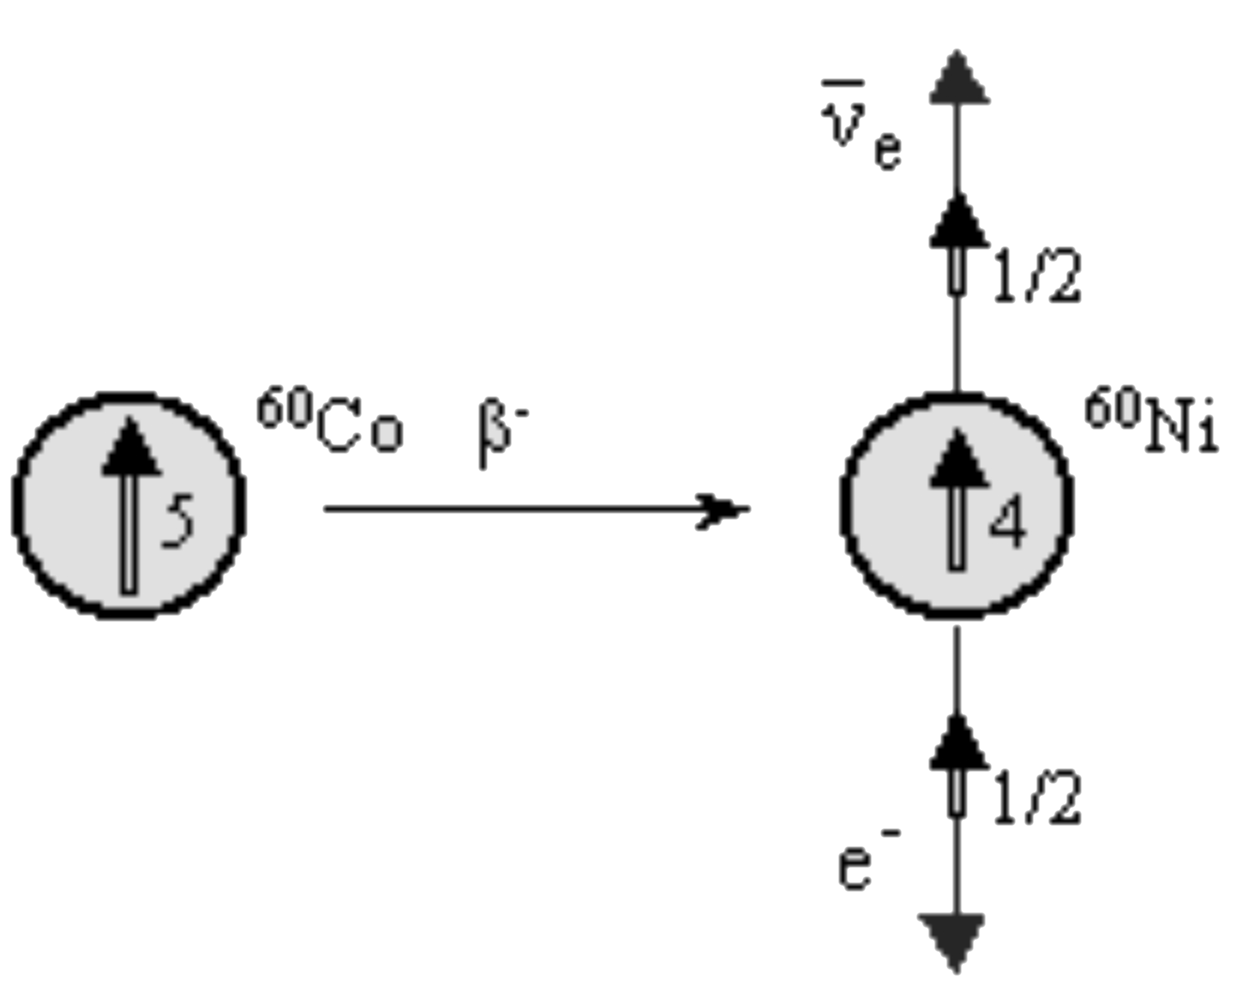
\includegraphics[width=1\linewidth]{p1.png}
    \caption{Схема опыта Ву} 
    \label{p1}
    \end{minipage}
    \hfill 
    \begin{minipage}[h]{0.4\linewidth}
    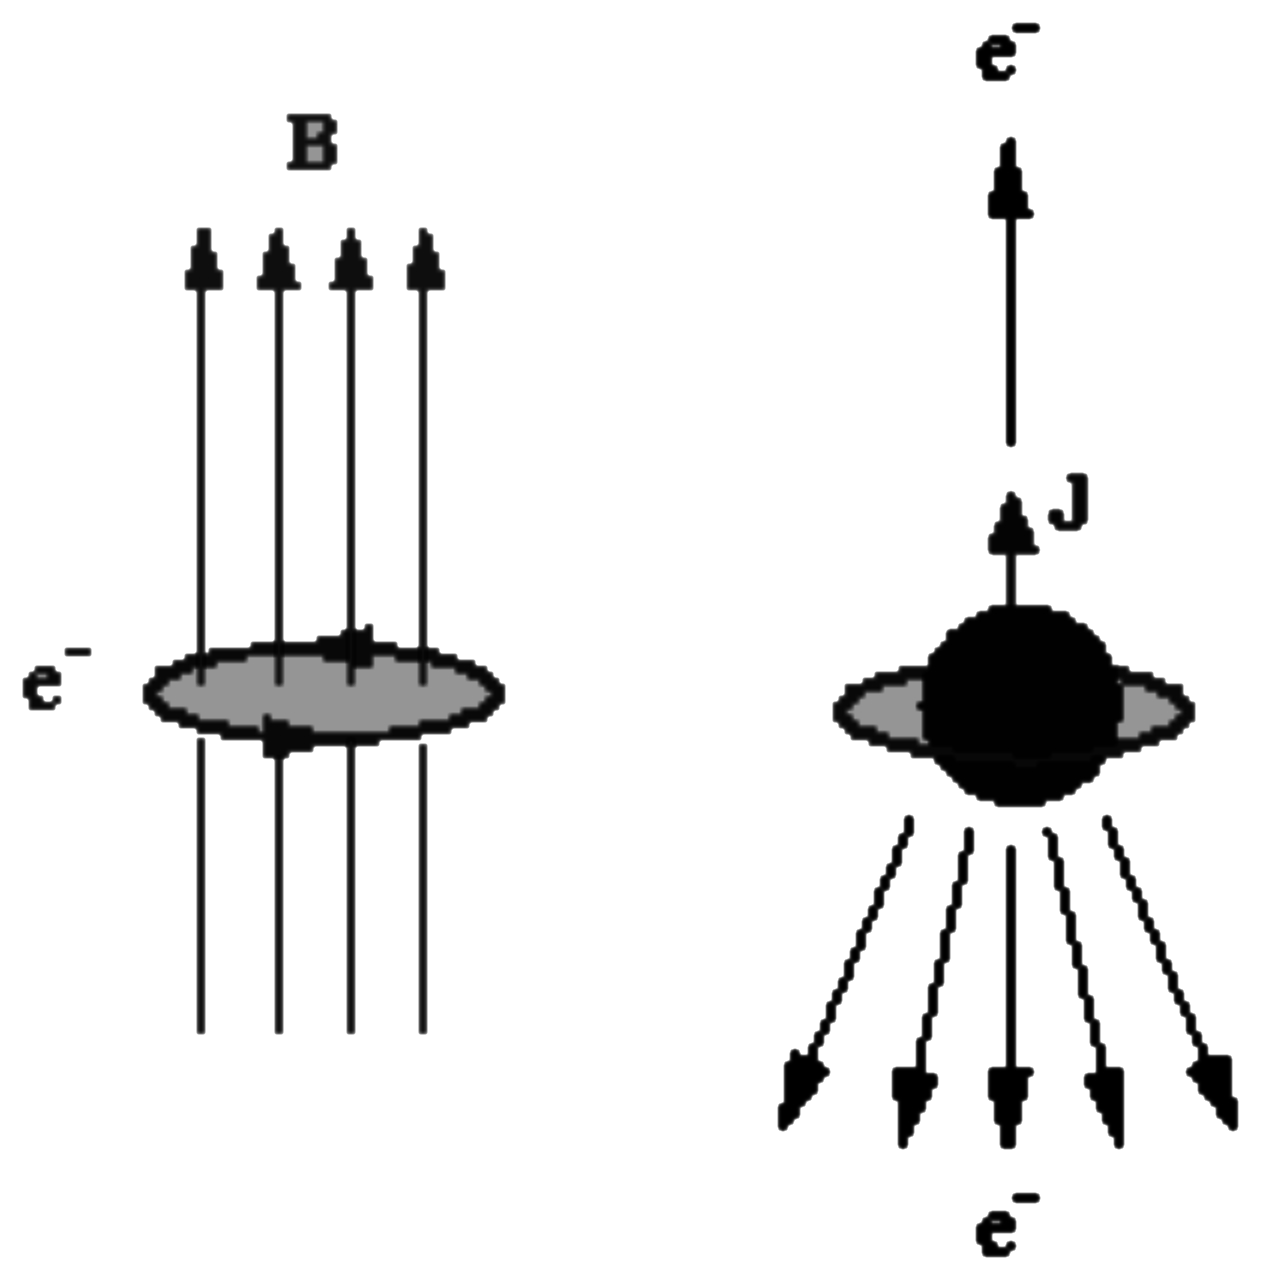
\includegraphics[width=1\linewidth]{p2.png}
    \caption{Орейнтации cпинов импульсов при $\beta^-$-распаде кобальта}
    \label{p2}
    \end{minipage}
    \end{center}
\end{figure}

Однако, оказалось  рис.\ref{p1}, что электроны испускаются преимущественно в направлении 
противоположном направлению магнитного поля (спинов ядер), тем самым было доказано, что в 
слабых распадах четность не сохраняется.

Спин у антинейтрино всегда направлен по импульсу (рис. \ref{p2}) (положительная или правая спиральность), 
у нейтрино против импульса (отрицательная или левая спиральность). При $\beta$-распаде сохраняется комбинированная 
CP-четность - последовательное применение пространственной и зарядовой инверсии (замене частиц на их античастицы (рис.\ref{p3})).

\begin{figure}[H]
    \begin{center}
    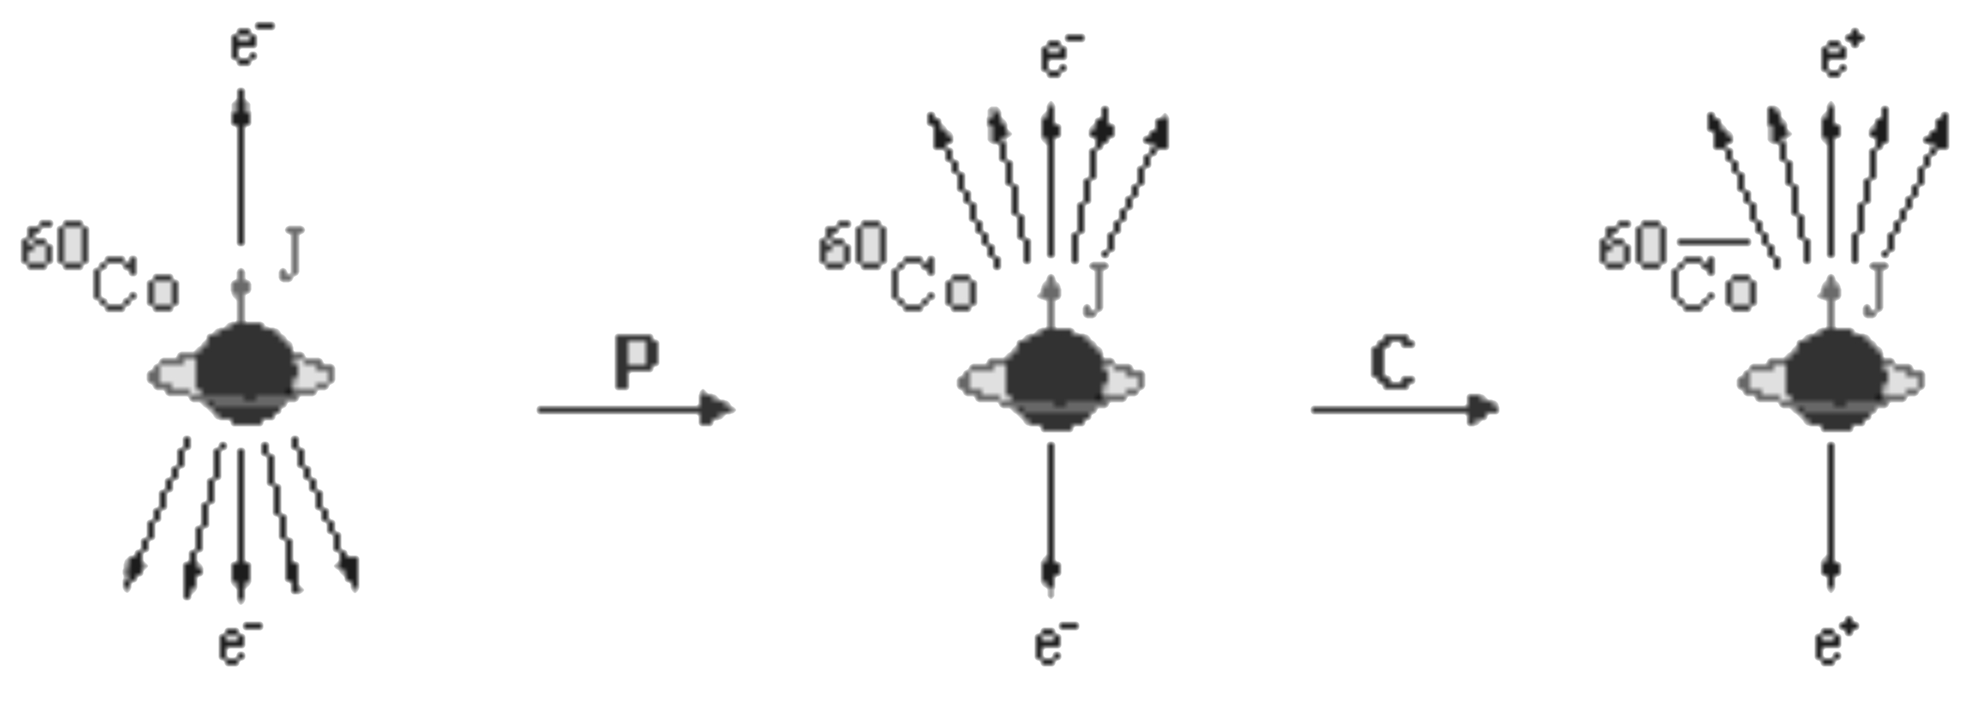
\includegraphics[scale = 0.2]{p3.png}
    \caption{CP - преобразование распада $^{60}Co$}
    \label{p3}
    \end{center}
\end{figure}

$\tilde{C}$ - оператор зарядового сопряжения

Частицу и античастицу отличают знаки электрического заряда $Q$, барионного числа $B$, лептонных чисел $L_e, L_{\mu}, L_{\tau}$, 
странности $s$, шарма $c$, красоты $b$, истины $t$. Операция зарядового сопряжения  переводит частицы в античастицы, 
т.е. меняет знаки зарядов, оставляя неизменными пространственные переменные $x$, импульс $p$ и момент импульса $J$.

$$x, p, J, Q, B, L_e, L_{\mu}, L_{\tau}, s, c, b, t \; \stackrel{\tilde{C}}{\rightarrow} \; x, p, J, -Q, -B, -L_e, -L_{\mu}, -L_{\tau}, -s, -c, -b, -t$$



\end{document}